\documentclass{article}

\usepackage{fancyhdr}
\usepackage{extramarks}
\usepackage{amsmath}
\usepackage{amsthm}
\usepackage{amsfonts}
\usepackage{tikz}
\usepackage[plain]{algorithm}
\usepackage{algpseudocode}
\usepackage{amssymb}
\usepackage{enumitem}
\usepackage{relsize}
\usepackage{textcomp}
\usepackage{graphicx}
\usepackage{bm}

\usetikzlibrary{automata,positioning}

%
% Basic Document Settings
%

\topmargin=-0.45in
\evensidemargin=0in
\oddsidemargin=0in
\textwidth=6.5in
\textheight=9.0in
\headsep=0.25in

\linespread{1.1}

\pagestyle{fancy}
\lhead{\hmwkAuthorName}
\chead{\hmwkClass\ (\hmwkClassInstructor\ \hmwkClassTime): \hmwkTitle}
\rhead{\hmwkDueDate}
\lfoot{\lastxmark}
\cfoot{\thepage}

\newcommand{\minus}{\scalebox{0.5}[1.0]{$-$}}
\newcommand\tab[1][0.5cm]{\hspace*{#1}}
\renewcommand\headrulewidth{0.4pt}
\renewcommand\footrulewidth{0.4pt}
\renewcommand{\theenumi}{\Alph{enumi}}

\setlength\parindent{0pt}

%
% Create Problem Sections
%

\newcommand{\enterProblemHeader}[1]{
	\nobreak\extramarks{}{{#1} continued on next page\ldots}\nobreak{}
	\nobreak\extramarks{{#1} (continued)}{{#1} continued on next page\ldots}\nobreak{}
}

\newcommand{\exitProblemHeader}[1]{
	\nobreak\extramarks{{#1} (continued)}{{#1} continued on next page\ldots}\nobreak{}
	\stepcounter{homeworkProblemCounter}
	\nobreak\extramarks{{#1}}{}\nobreak{}
}

\newcounter{homeworkProblemCounter}
\setcounter{secnumdepth}{0}
\newcounter{partCounter}
\nobreak\extramarks{Problem \arabic{homeworkProblemCounter}}{}\nobreak{}

%
% Homework Problem Environment
%
% This environment takes an optional argument. When given, it will adjust the
% problem counter. This is useful for when the problems given for your
% assignment aren't sequential. See the last 3 problems of this template for an
% example.
%
\newenvironment{homeworkProblem}[1][-1]{
	\subsection*{{#1}:}
	\enterProblemHeader{{#1}}
	\exitProblemHeader{{#1}}
}

%
% Homework Details
%   - Title
%   - Due date
%   - Class
%   - Section/Time
%   - Instructor
%   - Author
%

\newcommand{\hmwkTitle}{Chapter 1 Homework}
\newcommand{\hmwkDueDate}{September 09, 2019}
\newcommand{\hmwkClass}{MTH 5051}
\newcommand{\hmwkClassTime}{Section 01}
\newcommand{\hmwkClassInstructor}{Dr. Jim Jones}
\newcommand{\hmwkAuthorName}{\textbf{Eric Pereira}}

%
% Title Page
%
\pagenumbering{gobble}
\title{
	\vspace{2in}
	\textmd{\textbf{\hmwkClass:\ \hmwkTitle}}\\
	\normalsize\vspace{0.1in}\small{Due\ on\ \hmwkDueDate\ at 07:00pm}\\
	\vspace{0.1in}\large{\textit{\hmwkClassInstructor\ \hmwkClassTime}}
	\vspace{3in}
}

\author{\hmwkAuthorName}
\date{}

\renewcommand{\part}[1]{\textbf{\large Part \Alph{partCounter}}\stepcounter{partCounter}\\}

%
% Various Helper Commands
%

% Useful for algorithms
\newcommand{\alg}[1]{\textsc{\bfseries \footnotesize #1}}

% For derivatives
\newcommand{\deriv}[1]{\frac{\mathrm{d}}{\mathrm{d}x} (#1)}

% For partial derivatives
\newcommand{\pderiv}[2]{\frac{\partial}{\partial #1} (#2)}

% Integral dx
\newcommand{\dx}{\mathrm{d}x}

% Alias for the Solution section header
\newcommand{\solution}{\textbf{\large Solution}}

% Probability commands: Expectation, Variance, Covariance, Bias
\newcommand{\E}{\mathrm{E}}
\newcommand{\Var}{\mathrm{Var}}
\newcommand{\Cov}{\mathrm{Cov}}
\newcommand{\Bias}{\mathrm{Bias}}

\begin{document}
	
	\maketitle
	
	\pagebreak
	\pagenumbering{arabic}
	
	
	\section*{Sections 1.1-1.2}
	
	%%%%%%%%%%%%%%%%%%%%%%%%%%%%%%%%%%%%%%%%%%%%%%%%%%%%%%%%%%%%%%%%%%%%%%%%%%%%%%%%%%
	%                                                                                %
	%                        Sections 1.1-1.2 Problem 1                              %
	%                                                                                %
	%%%%%%%%%%%%%%%%%%%%%%%%%%%%%%%%%%%%%%%%%%%%%%%%%%%%%%%%%%%%%%%%%%%%%%%%%%%%%%%%%%
	\begin{homeworkProblem}[Problem 1]
		During a local campaign, eight Republican and five Democratic candidates are nominated for president of the school board.
		\begin{enumerate}[label=(\alph*)]
			\item If the president is to be one of these candidates, how many possibilites are there for the eventual winner?
			\item How many possibilities exist for a pair of candidates (one from each party) to oppose each other for the eventual
				election?
			\item Which counting principle is used in part (a)? in part (b)?\\
		\end{enumerate}
	

		\textbf{Solution:}
		\begin{enumerate}[label=(\alph*)]
			\item The possible winners essentially includes every candidate running within the group of Republicans and Democrats.
				Therefore, in order to see all possibilities you would add the amount of Republicans and Democrats.
				\begin{center}
					8 Republicans + 5 Democrats = \textbf{13 possible winners}
				\end{center}
			\item Each Republican candidate can face off against each Democratic candidate. Therefore, in order to see all possibilites
				for you would multiply the amount of Republicans by Democrats.
				\begin{center}
					8 Republicans $\times$ 5 Democrats = \textbf{40 possible candidate oppositions.} 
				\end{center}	
			\item in part (a) we use the \textbf{Rule of Sum}. In part (b) we use the \textbf{Rule of Product}
		\end{enumerate}
			
			
	\end{homeworkProblem}
	\newpage
	
	
	%%%%%%%%%%%%%%%%%%%%%%%%%%%%%%%%%%%%%%%%%%%%%%%%%%%%%%%%%%%%%%%%%%%%%%%%%%%%%%%%%%
	%                                                                                %
	%                        Sections 1.1-1.2 Problem 4                              %
	%                                                                                %
	%%%%%%%%%%%%%%%%%%%%%%%%%%%%%%%%%%%%%%%%%%%%%%%%%%%%%%%%%%%%%%%%%%%%%%%%%%%%%%%%%%
	
	\begin{homeworkProblem}[Problem 4]
		The board of directors of a pharmaceutical corporation has 10 members. An upcoming stockholders' meeting is scheduled
		to approve a new slate of company officers (chosen from the 10 board members).
		\begin{enumerate}[label=(\alph*)]
			\item How many different slates consisting of a president, vice president, secretary, and treasurer can the board present to
				the stockholders for their approval?
			\item Three members of the board of directors are physicians. How many slates from part (a) have 
			\begin{enumerate}[label=(\roman*)]
				\item A physician
				\item Exactly one physician appearing on the slate?
				\item At least one physician appearing on the slate?
			\end{enumerate}
		\end{enumerate}
	
		\textbf{Solution:}
		
		\begin{enumerate}[label=(\alph*)]
			\item This seems to be a permutation, where there are 10 total members on the board of directors and a new slate of company
				officers would consist of 4 people. The exact number would follow the equation:
				\begin{align*}
					\frac{n!}{(n-r)!}
				\end{align*}
				If we replace n with 10, the amount of board members, and r with 4, the amount of company officers needed on a new slate the
				different slates possible would be:
				\begin{align*}
					\frac{10!}{(10-4)!} = \bm{5040} \text{ \textbf{possible slates}}
				\end{align*}
			\item 
				\begin{enumerate}[label=(\roman*)]
					\item The amount of slates that include only a physician is another permutation. If we choose at least one
						physician for president, the equation would look like:
						\begin{center}
							3 physicians $\times$ 9 others $\times$ 8 others $\times$ 7 others = \\ \textbf{1512 slates with physicians
							nominated for president}
						\end{center}
					\item The amount of slates that include exactly one physician would look a bit different. In part (i) we allowed for 
						other physicians in the collection of the group, we have to subtract that. So the equation would look like:
						\begin{center}
							3 physicians $\times$ 7 non-physicans $\times$ 6 non-physicans $\times$ 5 non-physicans = \\ \textbf{630 slates
							with exactly one physician}
						\end{center}
					\item The easiest way to calculate this is to use a value we have, the total amount of possible slates, subtracted by
						the amount of slates without a physician.
						\begin{center}
							7 non-physicans $\times$ 6 non-physicans $\times$ 5 non-physicans $\times$ 4 non-physicans = \\ \textbf{840
							slates without a physician.} \\
							5040 total - 840 slates without physicans = \textbf{4200 slates with physicians}
						\end{center}
				\end{enumerate}
		\end{enumerate}	
	\end{homeworkProblem}
	\newpage
	
	%%%%%%%%%%%%%%%%%%%%%%%%%%%%%%%%%%%%%%%%%%%%%%%%%%%%%%%%%%%%%%%%%%%%%%%%%%%%%%%%%%
	%                                                                                %
	%                        Sections 1.1-1.2 Problem 9                              %
	%                                                                                %
	%%%%%%%%%%%%%%%%%%%%%%%%%%%%%%%%%%%%%%%%%%%%%%%%%%%%%%%%%%%%%%%%%%%%%%%%%%%%%%%%%%
	
	\begin{homeworkProblem}[Problem 9]
		Patter's Pastry Parlor offers eight different kinds of pastry and six different kinds of muffins. In addition to bakery items
		one can purchase small, medium, or large containers of the following beverages: coffee (black, with cream, with sugar, or with
		cream and sugar), tea (plain, with cream, with sugar, with cream and sugar, with lemon, or with lemon and sugar), hot cocoa, and
		orange juice. When Carol comes to Patter's, in how many ways can she order
		\begin{enumerate}[label=(\alph*)]
			\item One bakery item and one medium-sized beverage for herself?
			\item One bakery item and one container of coffee for herself and one muffin and one container of tea for her boss, Ms.
				Didio?
			\item One piece of pastry and one container of tea for herself, one muffin and a container of orange juice for Ms. Didio,
				and one bakery item and one container of coffee for each of her two assistants, Mr. Talbot and Mrs. Gillis? \\
		\end{enumerate}
		\textbf{Solution:}
		\begin{enumerate}[label=(\alph*)]
			\item There are a total of 14 bakery items (8 pastries + 6 muffins) and 12 options for drinks (if you count all the options for
				coffee and tea as  individual beverages). We would use the Rule of Products for this and get the value:
				\begin{center}
					14 bakery items $\times$ 12 different beverages = \textbf{168 combo options}
				\end{center}
			\item There are 14 total bakery items, 12 options for coffee beverage (3 sizes $\times$ 4 types of coffee), 6 muffins and
				and 18 different tea beverages (3 sizes $\times$ 6 types of tea.) This results in the equation:
				\begin{center}
					Carols Order: 14 bakery items $\times$ 12 coffee beverages = \textbf{168 options} \\
					Ms. Didio's Order: 6 Muffins $\times$ 18 tea beverages = \textbf{108 options} \\
					Total Order: 168 Options for Carol $\times$ 108 Options for Ms. Didio = \textbf{18,144 total options}
				\end{center}
			\item This is quite long to explain, I will let the equation do the talking:
				\begin{center}
					Carol's order: 8 pastries $\times$ 18 teas = \textbf{144 options} \\
					Ms. Didio's order: 6 muffins $\times$ 3 orange juices = \textbf{18 options} \\
					Assistants: (14 bakery items $\times$ 12 coffees)$^2$  = \textbf{28,224 options} \\
					Total: 144 Carol's options $\times$ 18 Ms. Didio's optoins $\times$ 28,224 other options = \textbf{73,156,608 options}
				\end{center}
		\end{enumerate}
	\end{homeworkProblem}
	\newpage
	
	%%%%%%%%%%%%%%%%%%%%%%%%%%%%%%%%%%%%%%%%%%%%%%%%%%%%%%%%%%%%%%%%%%%%%%%%%%%%%%%%%%
	%                                                                                %
	%                        Sections 1.1-1.2 Problem 19                             %
	%                                                                                %
	%%%%%%%%%%%%%%%%%%%%%%%%%%%%%%%%%%%%%%%%%%%%%%%%%%%%%%%%%%%%%%%%%%%%%%%%%%%%%%%%%%
	
	\begin{homeworkProblem}[Problem 19]
		A computer science professor has seven different programming books on a bookshelf. Three of the books deal with C++,
		the other four with Java. In how many ways can the professor arrange these books on the shelf
		\begin{enumerate}[label=(\alph*)]
			\item If there are no restrictions?
			\item If the languages should alternate? 
			\item If all the C++ books must be next to each other? 
			\item If all the C++ books must be next to each other and all the Java books must be next to each other?
		\end{enumerate}
		\textbf{Solution:}
		
		\begin{enumerate}[label=(\alph*)]
			\item If there are no restrictions then the solution is simply 7!. This value would be \textbf{5040}.
			\item If the books must alternate then there is only specific formation. The order would look like:
				\begin{center}
					Java, C++, Java, C++, Java, C++, Java.
				\end{center}
				From here we would have to see the possible ways to alternate the 4 different Java books and the 3 different C++ books. The 
				resulting solutiong would be:
				\begin{center}
					4! Java book configurations $\times$ 3! C++ book configurations = \textbf{144 possible configurations}
				\end{center}
			\item If all the C++ books have to be next to each other then there is 5 total configuration styles, they are:
				\begin{center}
					C++, C++, C++, Java, Java, Java, Java OR \\
					Java, C++, C++, C++, Java, Java, Java OR \\
					Java, Java, C++, C++, C++, Java, Java OR \\
					Java, Java, Java, C++, C++, C++, Java OR \\
					Java, Java, Java, Java, C++, C++, C++ 
				\end{center}
				Because of this, you would get the value from the possible amount of configurations and multiply it by 5:
				\begin{center}
					4! Java Configurations $\times$ 3! C++ configurations $\times$ 5 configuration styles = \textbf{720 arrangements}
				\end{center}
			\item There are only 2 configuration styles for this, those configuration styles are:
				\begin{center}
					Java, Java, Java, Java, C++, C++, C++ OR \\
					C++, C++, C++, Java, Java, Java, Java
				\end{center}
				Because of this, you would get the value from what the amount of possibilities from one of the configurations and double it.
				\begin{center}
					4! Java Configurations $\times$ 3! C++ configurations $\times$ 2 configurations styles = \textbf{288 
					arrangements}
				\end{center}
		\end{enumerate}
	\end{homeworkProblem}
	\newpage
	
	%%%%%%%%%%%%%%%%%%%%%%%%%%%%%%%%%%%%%%%%%%%%%%%%%%%%%%%%%%%%%%%%%%%%%%%%%%%%%%%%%%
	%                                                                                %
	%                        Sections 1.1-1.2 Problem 20                             %
	%                                                                                %
	%%%%%%%%%%%%%%%%%%%%%%%%%%%%%%%%%%%%%%%%%%%%%%%%%%%%%%%%%%%%%%%%%%%%%%%%%%%%%%%%%%
	
	\begin{homeworkProblem}[Problem 20]
		Over the Internet, data are transmitted in structured blocks of bits called \textit{datagrams}.
		\begin{enumerate}[label=(\alph*)]
			\item In how many ways can the letters in DATAGRAM be arranged?
			\item For the arrangements of part (a), how many have all three As together? \\
		\end{enumerate}
		\textbf{Solution:}
		\begin{enumerate}[label=(\alph*)]
			\item There are a total of 8 letters in DATAGRAM, however 3 of them happen to be A's. If we consider each A to be the same then
				we have to account for repeated words. There are a total of 8! combinations because there are 8 letters, and 3! combinations
				of repeated combinations because of the letter A. As a result we get:
				\begin{center}
					8! total combinations / 3! repeated combinations = \textbf{6720 arrangments}
				\end{center}
			\item If all 3 A's are together, there are a total arrangement of 6 different ways that they A's can be placed. There are a
				total of 5 letters other than the A's, so if the three A's Appear before the rest of the letters, and in between each, and after there are a total of 6 combinations. As a result the equation would look like:
				\begin{center}
					6! combinations = \textbf{720 arrangements}
				\end{center}
		\end{enumerate}
	\end{homeworkProblem}
	\newpage
	
	%%%%%%%%%%%%%%%%%%%%%%%%%%%%%%%%%%%%%%%%%%%%%%%%%%%%%%%%%%%%%%%%%%%%%%%%%%%%%%%%%%
	%                                                                                %
	%                        Sections 1.1-1.2 Problem 30                             %
	%                                                                                %
	%%%%%%%%%%%%%%%%%%%%%%%%%%%%%%%%%%%%%%%%%%%%%%%%%%%%%%%%%%%%%%%%%%%%%%%%%%%%%%%%%%
	
	\begin{homeworkProblem}[Problem 30]
		A sequence of letters of the form abcba, where the expression is unchanged upon reversing order, is an example of a
		palindrome (of five letters),
		\begin{enumerate}[label=(\alph*)]
			\item If a letter may appear more than twice, how many palindromes of five letters are there? of six letters? 
			\item Repeat part (a) under the condition that no letter appears more than twice.
		\end{enumerate}
		\textbf{Solution:}
		\begin{enumerate}[label=(\alph*)]
			\item There are 26 letters in the alphabet. In the case for 5 letters the first 2 letters have to match the last 2, the middle
				letter can be any letter and not matter. so for 5 letters the equation will look like:
				\begin{center}
					26 $\times$ 26 $\times$ 26 $\times$ 1 $\times$ 1 = \textbf{17,576 palindromes}
				\end{center}
				For 6 letters the first 3 letters have to be the same as the last 3. So the equation would look like:
				\begin{center}
					26 $\times$ 26 $\times$ 26 $\times$ 1 $\times$ 1 $\times$ 1 = \textbf{17,576 palindromes}
				\end{center}
				It's a big amusing that they both 5 letter and 6 letter words have the same amount of palindromes.
			\item In the case that no letter appears more than twice the amount of palindromes changes. It looks like:
				\begin{center}
					5 letters: 26 $\times$ 25 $\times$ 24 $\times$ 1 $\times$ 1 = \textbf{15,600 palindromes} \\
					6 letters: 26 $\times$ 25 $\times$ 24 $\times$ 1 $\times$ 1 $\times$ 1 = \textbf{15,600 palindromes}
				\end{center}
				
		\end{enumerate}
	\end{homeworkProblem}
	\newpage
	
	%%%%%%%%%%%%%%%%%%%%%%%%%%%%%%%%%%%%%%%%%%%%%%%%%%%%%%%%%%%%%%%%%%%%%%%%%%%%%%%%%%
	%                                                                                %
	%                        Sections 1.1-1.2 Problem 31                             %
	%                                                                                %
	%%%%%%%%%%%%%%%%%%%%%%%%%%%%%%%%%%%%%%%%%%%%%%%%%%%%%%%%%%%%%%%%%%%%%%%%%%%%%%%%%%
	\begin{homeworkProblem}[Problem 31]
		Determine the number of six-digit integers (no leading zeros) in which
		\begin{enumerate}[label=(\alph*)]
			\item No digit may be repeated
			\item Digits may be repeated
		\end{enumerate}
		Answer parts (a) and (b) with the extra condition that the six-digit integer is 
		\begin{enumerate}[label=(\roman*)]
			\item Even
			\item Divisible by 5
			\item Divisible by 4 \\
		\end{enumerate}
		\textbf{Solution:}
		\begin{enumerate}[label=(\alph*)]
			\item There are 9 numbers to choose from intially (1-9). After this we can include 0 in our choice of options, as there are no
				trailing zeroes if you are past the first number. If they all have to be different then the equation would look like:
				\begin{center}
					9 $\times$ 9 $\times$ 8 $\times$ 7 $\times$ 6 $\times$ 5 = \textbf{136,080 integers}
				\end{center}
				\begin{enumerate}[label=(\roman*)]
					\item you have to do two products here, one for numbers ending in 0 and one for numbers that end in 2,4,6,8. The 
						equation for this would look like:
						\begin{center}
							(9 $\times$ 8 $\times$ 7 $\times$ 6 $\times$ 5 $\times$ 1) ending in zero + (8 $\times$ 8 $\times$ 7 $\times$ 6
							$\times$ 5 $\times$ 4) ending in 2,4,6,8 = \textbf{68,800}
						\end{center}
					\item In this case we have to find numbers that end in 0 and 5. The equation would look like:
						\begin{center}
							(9 $\times$ 8 $\times$ 7 $\times$ 6 $\times$ 5 $\times$ 1) ending in zero + (8 $\times$ 8 $\times$ 7 $\times$ 6
							$\times$ 5 $\times$ 1) ending in 5 = \textbf{28,560}
						\end{center}
					\item Now, 4 is a bit different. 4 is not evenly divisible by 10, so we can't focus on just the last digit, it is 
						important to focus on the last 2 digits, as 4 is evenly divisible in 100. so any number that 4 evenly divides by in 
						the range 0-100 that does not include repeated values is what we are going to calculate. Now some of the numbers 
						that are divisible by 4 have a 0 in it; 04, 08, 20, 40, 60, 80. The rest of the numbers are; 12, 16, 24, 28, 32, 36,
						48, 52, 56, 64, 68, 72, 76, 84, 92, 96. The first list has 6 values, the second has 16. The equation would look
						like:
						\begin{center}
							(8 $\times$ 7 $\times$ 6 $\times$ 5 $\times$ 6) + (7 $\times$ 7 $\times$ 6 $\times$ 5 $\times$ 16) = \textbf{
							33,600}
						\end{center}
				\end{enumerate}
			\item If there are no leading zeroes and the numbers can be repeated, with no leading zeroes, you will get:
				\begin{center}
					9 $\times$ 10 $\times$ 10 $\times$ 10 $\times$ 10 $\times$ 10 = \textbf{900,000 integers}
				\end{center}
				\begin{enumerate}[label=(\roman*)]
					\item Essentially, the range of numbers is between 100,000 and 999,999 which actually means that there are the same
						amount of even numbers as there odd numbers. So, because of this, we can just divide the total integers by 2. 
						\begin{center}
							900,000 integers \ 2 = \textbf{450,000 integers}
						\end{center}
					\item Again, I am going to use a work around, but we can find all numbers divisible by 5 in this range by simply
						dividing by 5 (This only really works because 900,000 is divisible by 5, if 900,000 was divisible by 7, for
						example, this would not be the case, but if I can get the easy way to the right answer I will):
						\begin{center}
							900,000 integers \ 5 = \textbf{180,000 integers}
						\end{center}
					\item Again, I am going to use another work around, as 900,000 is divisible by 4. Here is the answer:
						\begin{center}
							900,000 integers \ 4 = \textbf{225,000 integers}
						\end{center}
				\end{enumerate}
		\end{enumerate}
	\end{homeworkProblem}
	\newpage
	
	%%%%%%%%%%%%%%%%%%%%%%%%%%%%%%%%%%%%%%%%%%%%%%%%%%%%%%%%%%%%%%%%%%%%%%%%%%%%%%%%%%
	%                                                                                %
	%                        Sectoin 1.3 Problem 3                                   %
	%                                                                                %	
	%%%%%%%%%%%%%%%%%%%%%%%%%%%%%%%%%%%%%%%%%%%%%%%%%%%%%%%%%%%%%%%%%%%%%%%%%%%%%%%%%%
	
	\section{Section 1.3}
	\begin{homeworkProblem}[Problem 3]
		Evaluate each of the following.
		\begin{enumerate}[label=(\alph*)]
			\item $C(10, 4)$
			\item $\binom{12}{7}$
			\item $C(14, 12)$
			\item $\binom{15}{10}$
		\end{enumerate}
		\textbf{Solution:}
		\begin{enumerate}[label=(\alph*)]
			\item 
				\begin{align*}
					\frac{10!}{(4!)(6!)} = \frac{10 \times 9 \times 8 \times 7}{4 \times 3 \times 2} = \bm{210}
				\end{align*}
			\item
				\begin{align*}
					\frac{12!}{(7!)(5!)} = \frac{12 \times 11 \times 10 \times 9 \times 8}{5 \times 4 \times 3 \times 2} = \bm{792}
				\end{align*} 
			\item 
				\begin{align*}
					\frac{14!}{(12!)(2!)} = \frac{14 \times 13}{2} = \bm{91}
				\end{align*}
			\item
				\begin{align*}
					\frac{15!}{(10!)(5!)} = \frac{15 \times 14 \times 13 \times 12 \times 11}{5 \times 4 \times 3 \times 2} = \bm{3003}
				\end{align*}
		\end{enumerate}
	\end{homeworkProblem}
	\newpage
	
	%%%%%%%%%%%%%%%%%%%%%%%%%%%%%%%%%%%%%%%%%%%%%%%%%%%%%%%%%%%%%%%%%%%%%%%%%%%%%%%%%%
	%                                                                                %
	%                        Sectoin 1.3 Problem 4                                   %
	%                                                                                %	
	%%%%%%%%%%%%%%%%%%%%%%%%%%%%%%%%%%%%%%%%%%%%%%%%%%%%%%%%%%%%%%%%%%%%%%%%%%%%%%%%%%
	\begin{homeworkProblem}[Problem 4]
		In the Braille system a symbol, such as a lowercase letter, punctuation mark, suffix, and so on, is given by raising at least
		one of the dots in the six-dot arrangement shown in part (a) of Fig. 1.7. (The six Braille positions are labeled in this part of
		the figure.) For example, in part (b) of the figure the dots in positions 1 and 4 are raised and this six-dot arrangement 
		represents the letter c. In parts (c) and (d) of the figure we have the representations for the letters m and t, respectively. 
		The definite article "the" is shown in part (e) of the figure, while part (f) contains the form for the suffix "ow." Finally, 
		the semicolon, ;, is given by the six-dot arrangement in part (g), where the dots at positions 2 and 3 are raised. 
		\begin{center}
			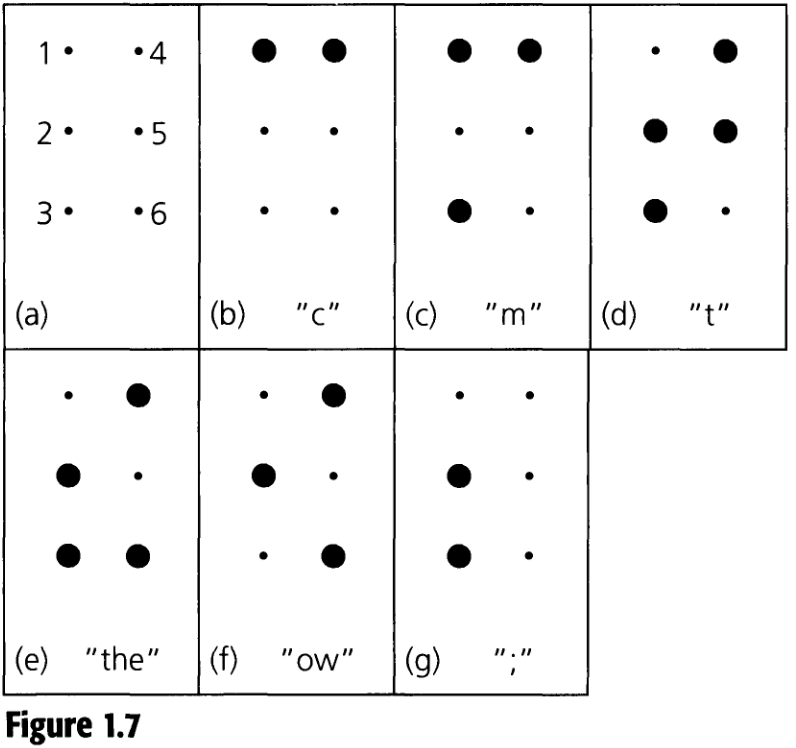
\includegraphics[scale=.4]{Figure17.png}\\
		\end{center}
	
		\begin{enumerate}[label=(\alph*)]
			\item How many different symbols can we represent in the Braille system? 
			\item How many symbols have exactly three raised dots?
			\item How many symbols have an even number of raised dots?
		\end{enumerate}
		
		\textbf{Solution:}
		\begin{enumerate}[label=(\alph*)]
			\item There are 2 states, much like a binary, of either raised or unraised. Therefore we would get:
				\begin{center}
					2$^{6 \text{ bumps}}$ - 1 empty state = \textbf{63 symbols}
				\end{center}
			\item This would be an n choose k problem, where n is 6 and k is 3. It would look like:
			\begin{align*}
				\binom{6}{3} = \frac{6!}{(3!)(3!)} = \frac{6 \times 5 \times 4}{3 \times 2} = \bm{20 \text{ \textbf{options with 3 raised
				dots}}}
			\end{align*}
			\item This equation would also be a binomial coefficient. I am not going to do all the math out for the binomial coefficients, 
			but, there are 3 even numbers we can choose from (2, 4, 6). The equation below shows:
			\begin{align*}
				\binom{6}{2} + \binom{6}{4} + \binom{6}{6} = \bm{31 \text{\textbf{ options for even number of raised dots}}} 
			\end{align*}
		\end{enumerate}
	\end{homeworkProblem}
	\newpage

	%%%%%%%%%%%%%%%%%%%%%%%%%%%%%%%%%%%%%%%%%%%%%%%%%%%%%%%%%%%%%%%%%%%%%%%%%%%%%%%%%%
	%                                                                                %
	%                        Sectoin 1.3 Problem 5                                   %
	%                                                                                %	
	%%%%%%%%%%%%%%%%%%%%%%%%%%%%%%%%%%%%%%%%%%%%%%%%%%%%%%%%%%%%%%%%%%%%%%%%%%%%%%%%%%

	\begin{homeworkProblem}[Problem 5]
		\begin{enumerate}[label=(\alph*)]
			\item How many permutations of size 3 can one produce with the letters m, r, a, f, and t?
			\item List all the combinations of size 3 that result for the letters m, r, a, f, and t. \\
		\end{enumerate}
		\textbf{Solution:}
		\begin{enumerate}[label=(\alph*)]
			\item If this is a permutation, you will get P(5, 3). This equation would look like:
				\begin{align*}
					\frac{5!}{(5-3)!} = \frac{5!}{2!} = 5 \times 4 \times 3 = \bm{60}
				\end{align*}
			\item Combinations mean that there would be no repeating combos (e.g (r,a,t) is equal to (a,r,t))
				\begin{align*}
					C(5,3) = \frac{5!}{(3!)((5-3)!)} = \frac{5!}{(3!)(2!)} = \frac{5 \times 4}{2} = \bm{10}
				\end{align*}
				To List them all: \\
				\begin{center}
					\begin{tabular}{c	c	c	c	c}
						m,r,a 	& m,r,f	 	& m,r,t 	& m,a,f 	& m,a,t \\
						m,f,t 	& r,a,f 	& r,a,t 	& r,f,t 	& a,f,t
					\end{tabular}
				\end{center}

		\end{enumerate}
	\end{homeworkProblem}
	\newpage
	
	%%%%%%%%%%%%%%%%%%%%%%%%%%%%%%%%%%%%%%%%%%%%%%%%%%%%%%%%%%%%%%%%%%%%%%%%%%%%%%%%%%
	%                                                                                %
	%                        Sectoin 1.3 Problem 8                                   %
	%                                                                                %	
	%%%%%%%%%%%%%%%%%%%%%%%%%%%%%%%%%%%%%%%%%%%%%%%%%%%%%%%%%%%%%%%%%%%%%%%%%%%%%%%%%%	
	
	\begin{homeworkProblem}[Problem 8]
		In how many ways can a gambler draw five cards from a standard deck and get
		\begin{enumerate}[label=(\alph*)]
			\item A flush (five cards of the same suit)?
			\item Four aces?
			\item Four of a kind?
			\item Three aces and two jacks?
			\item Three aces and a pair?
			\item A full house (three of a kind and a pair)?
			\item Three of a kind?
			\item Two pairs? \\
		\end{enumerate}
		\textbf{Solution:}
		\begin{enumerate}[label=(\alph*)]
			\item A standard deck has has 52 cards. Knowing this to get a flush it would have to choose 5 cards from the same suit. There 
				are 4 suits per deck, so that is choosing 5 out of 13. The proper equation for this would be:
				\begin{align*}
					\binom{13}{5} \times \binom{4}{1} = \bm{5,148}
				\end{align*}
			\item To get 4 aces you would choose 4 of 4 aces, and have one more card that can be any card in the deck. The equation would
				be:
				\begin{align*}
					\binom{4}{4} \times \binom{52-4}{1} = \bm{48}
				\end{align*}
			\item To get 4 of a kind is a bit different, there are a total of 13 possible 4 of a kinds in a deck, then you have to choose 
				1 from 48, and of course 4 from 4. The equation would look like:
				\begin{align*}
					\binom{13}{1} \times \binom{4}{4} \times \binom{48}{1} = \bm{628}
				\end{align*}	
			\item There are 4 aces and 4 jacks. So you would choose 3 from 4 aces and choose 2 from 4 jacks. The equation would look like:
				\begin{align*}
					\binom{4}{3} \times \binom{4}{2} = \bm{24}
				\end{align*}
			\item There are a total of 13 possible pairs, but because we have 3 aces we would have to subtract 1 of the pairs possible.
				This would be 4 choose 3 aces and 12 choose 1 ranks and of each rank you would have 4 choose 2. This would look like:
				\begin{align*}
					\binom{4}{3} \times \binom{12}{1} \times \binom{4}{2} = \bm{288}
				\end{align*}
			\item There are 13 ranks, and if we want one to be a three of a kind we have to choose 1 of these 13, and 3 of the 4 cards per 
				rank. After this you would have 12 ranks left, and choose 1 of them and choose 2 from 4. This equation would look like:
				\begin{align*}
					\binom{13}{1} \times \binom{4}{3} \times \binom{12}{1} \times \binom{4}{2} = \bm{3,744}
				\end{align*}
			\item a three of a kind means we choose 1 from 13, and 3 from 4. After this we have two cards left to choose, so we would 
				ideally choose 2 from 48 however we can't risk matching a pair so we have to make sure that, luckily we can use the value
				from part (e) that specifies all amounts with three aces and a pair. Easy, the equation would look like:
				\begin{align*}
					(\binom{13}{1} \times \binom{4}{3} \times \binom{48}{2}) - 3,744 = \bm{58,656}
				\end{align*}
			\item Choosing two pairs means I choose 1 from 13, and 2 from those 4. Then I choose 1 from 12, and 2 from those 4. This leaves
				44 cards that we can choose from without causing a three of a kind, this equation looks like:
				\begin{align*}
					\binom{13}{1} \times \binom{4}{2} \times \binom{12}{1} \times \binom{4}{2} \times \binom{44}{1} = \bm{247,104} 
				\end{align*}
		\end{enumerate}
	\end{homeworkProblem}
	\newpage
	
	%%%%%%%%%%%%%%%%%%%%%%%%%%%%%%%%%%%%%%%%%%%%%%%%%%%%%%%%%%%%%%%%%%%%%%%%%%%%%%%%%%
	%                                                                                %
	%                        Sectoin 1.3 Problem 11                                  %
	%                                                                                %	
	%%%%%%%%%%%%%%%%%%%%%%%%%%%%%%%%%%%%%%%%%%%%%%%%%%%%%%%%%%%%%%%%%%%%%%%%%%%%%%%%%%
	
	\begin{homeworkProblem}[Problem 11]
		A student is to answer seven out of 10 questions on an examination. In how many ways can he make his selection if
		\begin{enumerate}[label=(\alph*)]
			\item There are no restrictions?
			\item He must answer the first two questions?
			\item He must answer at least four of the first six questions? \\
		\end{enumerate}
		\textbf{Solution:}
		\begin{enumerate}[label=(\alph*)]
			\item You just choose 7 from 10. The equation would look like:
				\begin{align*}
					\binom{10}{7} = \bm{120}
				\end{align*}
			\item If you must answer the first 2 questions this reduced the total options of other selections down to 8, and answers left
				out of 5. This would be:
				\begin{align*}
					\binom{8}{5} = \bm{56}
				\end{align*}
			\item  in this case we have many options. At minimum we have to answer 4 of the first 6, however we could answer 5, or all 6. 
				This causes the situation to be a bit tricky, but all we really have to do is multiply is the value of 4 choose 6 by the 
				value of 4 choose (7-4) for each card after, and follow a similar trend with 5 and 6. It's probably easier to see in an 
				equation:
				\begin{align*}
					\left( \binom{6}{4} \times \binom{4}{3} \right) + \left(\binom{6}{5} \times \binom{4}{2}\right) + 
					\left(\binom{6}{6} \times \binom{4}{1}\right) = \bm{100}
				\end{align*}
		\end{enumerate}
	\end{homeworkProblem}
	\newpage

	%%%%%%%%%%%%%%%%%%%%%%%%%%%%%%%%%%%%%%%%%%%%%%%%%%%%%%%%%%%%%%%%%%%%%%%%%%%%%%%%%%
	%                                                                                %
	%                        Sectoin 1.3 Problem 17                                  %
	%                                                                                %	
	%%%%%%%%%%%%%%%%%%%%%%%%%%%%%%%%%%%%%%%%%%%%%%%%%%%%%%%%%%%%%%%%%%%%%%%%%%%%%%%%%%

	\begin{homeworkProblem}[Problem 17]
		Express each of the following using the summation (or Sigma) notation. In parts (a), (d), and (e), n denotes a positive integer.
		\begin{enumerate}[label=(\alph*)]
			\item $\frac{1}{2!}+\frac{1}{3!}+\frac{1}{4!}+...+\frac{1}{n!}, n \ge 2$
			\item $1+4+9+16+25+49+64$
			\item $1^3-2^3+3^3-4^3+5^3-6^3+7^3$
			\item $\frac{1}{n}+\frac{2}{n+1}+\frac{3}{n+2}+...+\frac{n+1}{2n}$
			\item $n-(\frac{n+1}{2!})+(\frac{n+2}{4!})-(\frac{n+3}{6!})+...+(-1)(\frac{2n}{(2n)!})$
		\end{enumerate}
		\textbf{Solution:}
		\begin{enumerate}[label=(\alph*)]
			\item 
				\begin{align*}
					\sum_{i=2}^{n} \frac{1}{i!}
				\end{align*}
			\item 
				\begin{align*}
					\sum_{i=1}^{n} i^2
				\end{align*}
			\item 
				\begin{align*}
					\sum_{i=1}^{n} (-1)^{i+1} \times i^3
				\end{align*}
			\item 
				\begin{align*}
					\sum_{i=0}^{n} \frac{i + 1}{n+i}
				\end{align*}
			\item
				\begin{align*}
					\sum_{i=0}^{n} (-1)^{i} \times \frac{n+i}{2i!}
				\end{align*}
		\end{enumerate}
	\end{homeworkProblem}
	\newpage

	%%%%%%%%%%%%%%%%%%%%%%%%%%%%%%%%%%%%%%%%%%%%%%%%%%%%%%%%%%%%%%%%%%%%%%%%%%%%%%%%%%
	%                                                                                %
	%                        Sectoin 1.3 Problem 20                                  %
	%                                                                                %	
	%%%%%%%%%%%%%%%%%%%%%%%%%%%%%%%%%%%%%%%%%%%%%%%%%%%%%%%%%%%%%%%%%%%%%%%%%%%%%%%%%%

	\begin{homeworkProblem}[Problem 20]
		In the three parts of Fig. 1.8, eight points are equally spaced and marked on the circumference of a given circle.
		\begin{center}
			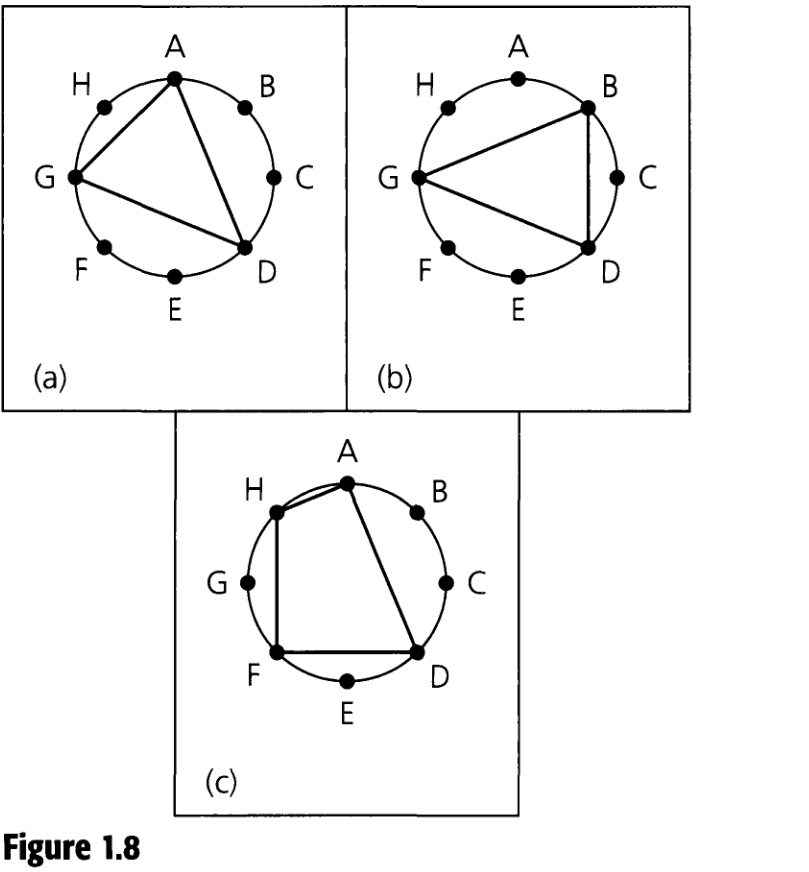
\includegraphics[scale=.4]{Figure18.png}
		\end{center}
	\begin{enumerate}[label=(\alph*)]
		\item For parts (a) and (b) of Fig. 1.8 we have two different(though congruent) triangles. These two triangles (distinguished 
		by their vertices) result from two selections of size 3 from the vertices A, B, C, D, E, F, G, H. How many different (whether
		congruent or not) triangles can we inscribe in the circle in this way?
		\item How many different quadrilaterals can we inscribe in the circle, using the marked vertices? [One such quadrilateral
		appears in part (c) of Fig. 1.8.]
		\item How many different polygons of three or more sides can we inscribe in the given circle by using three or more of the
		marked vertices? \\
	\end{enumerate}
		\textbf{Solution:}
		\begin{enumerate}[label=(\alph*)]
			\item If there are 8 points, and we have to select 3 for a triangle it is a simple 8 choose 3 binomial coefficient:
				\begin{align*}
					\binom{8}{3} = \bm{56}
				\end{align*}
			\item If we are doing quadrilaterals we just choose 4 instead of 3 similar to (a):
				\begin{align*}
					\binom{8}{4} = \bm{70}
				\end{align*}
			\item In this case you have to add all the values from 3-8 using binomial coefficients, the equation below shows this:
				\begin{align*}
					\binom{8}{3} + \binom{8}{4} + \binom{8}{5} + \binom{8}{6} + \binom{8}{7} + \binom{8}{8} = \bm{219}
				\end{align*}
		\end{enumerate}
	\end{homeworkProblem}
	\newpage

	%%%%%%%%%%%%%%%%%%%%%%%%%%%%%%%%%%%%%%%%%%%%%%%%%%%%%%%%%%%%%%%%%%%%%%%%%%%%%%%%%%
	%                                                                                %
	%                        Sectoin 1.3 Problem 21                                  %
	%                                                                                %	
	%%%%%%%%%%%%%%%%%%%%%%%%%%%%%%%%%%%%%%%%%%%%%%%%%%%%%%%%%%%%%%%%%%%%%%%%%%%%%%%%%%

	\begin{homeworkProblem}[Problem 21]
		How many triangles are determined by the vertices of a regular polygon of $n$ sides? How many if no side of the polygon
		is to be a side of any triangle? \\
		\textbf{Solution:} \\
		For a polygon of $n$ vertices there are $\binom{n}{3}$ for the three sides. now, if no side of the polygon is to be a side of any
		triangle, this provides a bit more of an issue. The easiest way to find the answer to this is to subtract all possible triangles 
		with edges that are one of the shapes of the n-sided polygon. This would result in the equation:
		\begin{align*}
			\binom{n}{3} - n \text{ sides} - n(n-4) \text{ shapes with one side}
		\end{align*}
	\end{homeworkProblem}
	\newpage
		
	%%%%%%%%%%%%%%%%%%%%%%%%%%%%%%%%%%%%%%%%%%%%%%%%%%%%%%%%%%%%%%%%%%%%%%%%%%%%%%%%%%
	%                                                                                %
	%                        Sectoin 1.4 Problem 1                                   %
	%                                                                                %	
	%%%%%%%%%%%%%%%%%%%%%%%%%%%%%%%%%%%%%%%%%%%%%%%%%%%%%%%%%%%%%%%%%%%%%%%%%%%%%%%%%%
	
	\section{Section 1.4}
	\begin{homeworkProblem}[Problem 1]
		In how many ways can 10 (identical) dimes be distributed among five children if
		\begin{enumerate}[label=(\alph*)]
			\item There are no restrictions?
			\item Each child gets at least one dime? 
			\item The oldest child gets at least two dimes?
		\end{enumerate}
		\textbf{Solution:}
		\begin{enumerate}[label=(\alph*)]
			\item This is a permutation with repetition, so the equation for these types of questions look like:
				\begin{align*}
					\frac{(n+r-1)!}{r!(n-1)!} = \binom{n+r-1}{r}
				\end{align*}
				In this case the problem has 5 as its n value, the amount of children, and r is the repeated value, the amount of dimes,
				10. This equation would look like:
				\begin{align*}
					\frac{(5+10-1)!}{10!(5-1)!} = \binom{5+10-1}{10} = \binom{14}{10} = \bm{1,001}
				\end{align*}
			\item In this case the r value becomes 5 because each child needs to have at least 1 coin. This means that we do the equation 
				previously, but replace all r values with 5. 
				\begin{align*}
					\frac{(5+5-1)!}{5!(5-1)!} = \binom{5+5-1}{5} = \binom{9}{5} = \bm{126}
				\end{align*}
			\item We subtract 2 from 10, and have 8 as our repetition value. We do the same equation as before.
				\begin{align*}
					\frac{(5+8-1)!}{8!(5-1)!} = \binom{5+8-1}{8} = \binom{12}{8} = \bm{495}
				\end{align*}
		\end{enumerate}
	\end{homeworkProblem}
	\newpage
	
	%%%%%%%%%%%%%%%%%%%%%%%%%%%%%%%%%%%%%%%%%%%%%%%%%%%%%%%%%%%%%%%%%%%%%%%%%%%%%%%%%%
	%                                                                                %
	%                        Sectoin 1.4 Problem 4                                   %
	%                                                                                %	
	%%%%%%%%%%%%%%%%%%%%%%%%%%%%%%%%%%%%%%%%%%%%%%%%%%%%%%%%%%%%%%%%%%%%%%%%%%%%%%%%%%
	
	\begin{homeworkProblem}[Problem 4]
		A certain ice cream store has 31 flavors of ice cream available. In how many ways can we order a dozen ice cream cones if
		\begin{enumerate}[label=(\alph*)]
			\item We do not want the same flavor more than once?
			\item A flavor may be ordered as many as 12 times?
			\item A flavor may be ordered no more than 11 times?
		\end{enumerate} 
		\textbf{Solution:}
		\begin{enumerate}[label=(\alph*)]
			\item This is simple, we need to choose 12 different flavors from 31 options:
				\begin{align*}
					\binom{31}{12} = \bm{141,120,525}
				\end{align*}
			\item This model includes repetiton, where the r value is 12 and the n value is 31. The equation is:
				\begin{align*}
					\binom{31+12-1}{12}=\binom{42}{12}=\bm{11,058,116,888}
				\end{align*}
			\item The easy way to do this is to get the previous value, the total value of all possible combinations that can have repeating
				flavors, but subtract the amount of orders that have all 12 ice creams being the same flavor. This would be:
				\begin{align*}
					11,058,116,888 - \binom{31}{1} = \bm{11,058,116,857}
				\end{align*}
		\end{enumerate}
	\end{homeworkProblem}
	\newpage
	
	%%%%%%%%%%%%%%%%%%%%%%%%%%%%%%%%%%%%%%%%%%%%%%%%%%%%%%%%%%%%%%%%%%%%%%%%%%%%%%%%%%
	%                                                                                %
	%                        Sectoin 1.4 Problem 7                                   %
	%                                                                                %	
	%%%%%%%%%%%%%%%%%%%%%%%%%%%%%%%%%%%%%%%%%%%%%%%%%%%%%%%%%%%%%%%%%%%%%%%%%%%%%%%%%%
	
	\begin{homeworkProblem}[Problem 7]
		Determine the number of integer solutions of
		\begin{align*}
			x_1+x_2+x_3+x_4=32,
		\end{align*}
		where
		\begin{enumerate}[label=(\alph*)]
			\item $x_i \ge 0, \quad 1\le i\le 4$
			\item $x_i > 0, \quad 1\le i\le 4$
			\item $x_1,x_2\ge 5, \quad x_3,x_4\ge 7$
			\item $x_i \ge 8, \quad 1\le i\le 4$
			\item $x_i\ge -2, \quad 1\le i \le 4$
			\item $x_1,x_2,x_3>0, \quad 0<x_4\le 25$
		\end{enumerate}
		\textbf{Solution:}
		\begin{enumerate}[label=(\alph*)]
			\item This is a permutation with repetition, where the r value is the value of all numbers, 32, and the n value is 4, the amount
				of variables. This would look like:
				\begin{align*}
					\binom{32+4-1}{32} = \binom{35}{32} = \bm{6,545}
				\end{align*}
			\item This is another repetiton, except each value has to equal at least 1. This means the max r value is 28, as 32 - 4 (4 
			being the total of the minimum of integers added up) = 28. the n value is still 4, for the amount of variables.
				\begin{align*}
					\binom{28+4-1}{28} = \binom{31}{28} = \bm{4,495}
				\end{align*}
			\item We are going to do something similar to before, we are getting the minimum value of all the variables added together and
				subtracting that from the total: 32. This is 32-10-14=8. 8 is our new r value.
				\begin{align*}
					\binom{8+4-1}{8} = \binom{11}{8} = \bm{165}
				\end{align*}
			\item There is actually only 1 solution to this. If all values are $\ge$ to 8 and there are 4 numbers, and they add up to
				32 then there is only 1 possible solution. 32/4=8. All values would have to be 8, so there is only \textbf{1 integer
				solution}
			\item The minimum value here is a bit different, in fact the new r value would be 32-(-8) = 40, the n value is still 4. This 
				results in the value:
				\begin{align*}
					\binom{40+4-1}{40} = \binom{43}{40} = \bm{12,341}
				\end{align*}
			\item I think the easiest way to get this problem is to get the value stated in part (b) and subtract that from any value where
				$x_4 \ge 26$. This equation would look like:
				\begin{align*}
					4,495 - \binom{6}{3} = \bm{4,475}
				\end{align*}
		\end{enumerate}
	\end{homeworkProblem}
	\newpage
	
	%%%%%%%%%%%%%%%%%%%%%%%%%%%%%%%%%%%%%%%%%%%%%%%%%%%%%%%%%%%%%%%%%%%%%%%%%%%%%%%%%%
	%                                                                                %
	%                        Sectoin 1.4 Problem 10                                  %
	%                                                                                %	
	%%%%%%%%%%%%%%%%%%%%%%%%%%%%%%%%%%%%%%%%%%%%%%%%%%%%%%%%%%%%%%%%%%%%%%%%%%%%%%%%%%
	
	\begin{homeworkProblem}[Problem 10]
		In how many ways can Lisa toss 100 (identical) dice so that at least three of each type of face will be showing? \\
		\textbf{Solution:} \\
		There are a total of 6 different sides of a dice, assuming that you have at least 3 of each side 18 dice, and there are 100 dice. 
		this would be a permutation with repetition, so we would get the 100 dice and subtract 18 from that. The n value is the 6 sides of
		the dice, and the r value is the 82 dice left over. The equation would then be:
		\begin{align*}
			\binom{82+6-1}{82} = \binom{87}{82} = \bm{36,949,857}
		\end{align*}
	\end{homeworkProblem}
	\newpage
	
	%%%%%%%%%%%%%%%%%%%%%%%%%%%%%%%%%%%%%%%%%%%%%%%%%%%%%%%%%%%%%%%%%%%%%%%%%%%%%%%%%%
	%                                                                                %
	%                        Sectoin 1.4 Problem 12                                  %
	%                                                                                %	
	%%%%%%%%%%%%%%%%%%%%%%%%%%%%%%%%%%%%%%%%%%%%%%%%%%%%%%%%%%%%%%%%%%%%%%%%%%%%%%%%%%
	
	\begin{homeworkProblem}[Problem 12]
		Determine the number of integer solutions of
		\begin{align*}
			x_1+x_2+x_3+x_4 + x_5 < 40
		\end{align*}
		where
		\begin{enumerate}[label=(\alph*)]
			\item $x_i \ge 0, \quad 1\le i\le 5$
			\item $x_i\ge -3 \quad 1\le i\le 5$
		\end{enumerate}
		\textbf{Solution:}
		\begin{enumerate}[label=(\alph*)]
			\item This problem is equal to the problem $x_1+x_2+x_3+x_4+x_5 \le 39$. Now there are quite a few equations here, but this
				can be simplified even further, we can say $x_1+x_2+x_3+x_4+x_5+x_6 = 39, \quad x_i \ge 0, \quad 0 \le i \le 6$ Where we 
				add another variable. From here it is a repetetive permutation, where n is the variables (5) and r is the value needed for
				them to add up to, 39. 
				\begin{align*}
					\binom{39+6-1}{39} = \binom{44}{39} = \bm{1,086,008}
				\end{align*}
			\item We are doing the same thing as before, except we have to change our r value. It will no longer be 39, but it will be 57
				because we have to consider the aboslute minimum possible value of all numbers, and append the difference 39. The equation
				then looks like:
				\begin{align*}
					\binom{57+6-1}{57} = \binom{62}{57} = \bm{6,471,002}
				\end{align*} 
		\end{enumerate}
	\end{homeworkProblem}
	\newpage
	
	%%%%%%%%%%%%%%%%%%%%%%%%%%%%%%%%%%%%%%%%%%%%%%%%%%%%%%%%%%%%%%%%%%%%%%%%%%%%%%%%%%
	%                                                                                %
	%                        Sectoin 1.4 Problem 13                                  %
	%                                                                                %	
	%%%%%%%%%%%%%%%%%%%%%%%%%%%%%%%%%%%%%%%%%%%%%%%%%%%%%%%%%%%%%%%%%%%%%%%%%%%%%%%%%%

	\begin{homeworkProblem}[Problem 13]
		In how many ways can we distribute eight identical white balls into four distinct containers so that
		\begin{enumerate}[label=(\alph*)]
			\item No container is left empty?
			\item The fourth container has an odd number of balls in it? \\
		\end{enumerate}
		\textbf{Solution:}
		\begin{enumerate}[label=(\alph*)]
			\item each container has to have at least 1 ball if you don't want any container to be empty. This means at least 1 ball per
				container. This means that the r value for the balls is 4 and the containers is the n value at 4. For a repetitive
				permutation this equation would be:
				\begin{align*}
					\binom{4+4-1}{4} = \binom{7}{4} = \bm{35}
				\end{align*}
			\item if the fourth container has an odd number of balls it has either 1, 3, 5, or 7 balls, for a total of 4 possibilities. The
			n value for these will be 3 to seaparate the other 3 containers excluding the 4th container. In each case the number of
			repetitive permutations is different, the equation would look like:
				\begin{align*}
					\binom{3+7-1}{7} + \binom{3+5-1}{5} + \binom{3+3-1}{3} + \binom{3+1-1}{1} = \bm{70}
				\end{align*}
		\end{enumerate}
	\end{homeworkProblem}
	\newpage
	
	%%%%%%%%%%%%%%%%%%%%%%%%%%%%%%%%%%%%%%%%%%%%%%%%%%%%%%%%%%%%%%%%%%%%%%%%%%%%%%%%%%
	%                                                                                %
	%                        Sectoin 1.4 Problem 17                                  %
	%                                                                                %
	%%%%%%%%%%%%%%%%%%%%%%%%%%%%%%%%%%%%%%%%%%%%%%%%%%%%%%%%%%%%%%%%%%%%%%%%%%%%%%%%%%	
	
	\begin{homeworkProblem}[Problem 17]
		How many ways are there to place 12 marbles of the same size in five distinct jars if 
		\begin{enumerate}[label = (\alph*)]
			\item The marbles are all black?
			\item each marble is a different color?
		\end{enumerate}
		\textbf{Solution:}
		\begin{enumerate}[label = (\alph*)]
			\item This is a repetitive permutation, where the 5 jars is n and the 12 marbles are r values. The equation would look like:
				\begin{align*}
					\binom{12+5-1}{12} = \binom{16}{12} = \bm{1,820}
				\end{align*}
			\item If each marble is a different color, and there are 5 jars, you simply have $\bm{5^{12}}$ \textbf{placements} 
		\end{enumerate}
	\end{homeworkProblem}
	\newpage
	
	%%%%%%%%%%%%%%%%%%%%%%%%%%%%%%%%%%%%%%%%%%%%%%%%%%%%%%%%%%%%%%%%%%%%%%%%%%%%%%%%%%
	%                                                                                %
	%                        Sectoin 1.4 Problem 23                                  %
	%                                                                                %
	%%%%%%%%%%%%%%%%%%%%%%%%%%%%%%%%%%%%%%%%%%%%%%%%%%%%%%%%%%%%%%%%%%%%%%%%%%%%%%%%%%		
	
	\begin{homeworkProblem}[Problem 23]
		\begin{enumerate}[label=(\alph*)]
			\item Given positive integers $m$, $n$ with $m \ge n$, show that the number of ways to distribute $m$ identical objects into
					$n$ distinct containers with no container left empty is
				\begin{align*}
					C(m-1,m-n) = C(m-1,n-1).
				\end{align*}
			\item Show that the number of distributions in part (a) where each container holds at least $r$ objects ($m \ge nr$) is
				\begin{align*}
					C(m-1+A-r)n,n-1).
				\end{align*}
		\end{enumerate}
		\textbf{Solution:}
		\begin{enumerate}[label=(\alph*)]
			\item If you put one object in each container you'll get a repetitive permutation for the rest of your objects, this will look
				like:
				\begin{align*}
					\binom{n+(m-n)-1}{m-n} = \binom{m-1}{m-n} = \binom{m-1}{n-1}
				\end{align*}
				Which proves the statement mentioned true.
			\item Next is using distributions for part (a) but each container holds at least r objects. The equation is similar to the 
				above, but differs slightly. The equation is as follows:
				\begin{align*}
					\binom{n+(m-rn)-1}{m-rn} = \binom{(m-1)+(1-r)n}{m-rn} = \binom{(m-1)+(1-r)n}{n-1}
				\end{align*}
		\end{enumerate}
	\end{homeworkProblem}
	\newpage
	
	%%%%%%%%%%%%%%%%%%%%%%%%%%%%%%%%%%%%%%%%%%%%%%%%%%%%%%%%%%%%%%%%%%%%%%%%%%%%%%%%%%
	%                                                                                %
	%                        Sectoin 1.4 Problem 23                                  %
	%                                                                                %
	%%%%%%%%%%%%%%%%%%%%%%%%%%%%%%%%%%%%%%%%%%%%%%%%%%%%%%%%%%%%%%%%%%%%%%%%%%%%%%%%%%	
	
	\begin{homeworkProblem}[Problem 27]
		Frannie tosses a coin 12 times and gets five heads and seven tails. In how many ways can these tosses result in
		\begin{enumerate}[label=(\alph*)]
			\item Two runs of heads and one run of tails; 
			\item Three runs;
			\item Four runs;
			\item Five runs;
			\item Six runs; and
			\item Equal numbers of runs of heads and runs of tails?
		\end{enumerate}
		\textbf{Solution:}
		\begin{enumerate}[label=(\alph*)]
			\item If we have 7 tails, the single run of tails is 7 tails long. This means that there is a portion of heads that happens 
				before and after this run. It has to be at least one heads to be considered a run, due to such the r value is 3 (the 
				floating heads we have available to cause changes) and 2 for n, the amount of heads streaks:
				\begin{align*}
					\binom{2+3-1}{3}=\binom{4}{3}=\bm{4}
				\end{align*}
			\item We already figured out one of the three run configurations in (a), we need to add that to a run that is THT. That would 
				look like this in an equation:
				\begin{align*}
					4+\binom{2+5-1}{5}=4+6=\bm{10}
				\end{align*}
			\item For four runs we could have a HTHT configuration, or a THTH configuration, so we would multiply head tails 
			calculations and multiply by 2 for each configuration. This would be defined by the calculation below:
				\begin{align*}
					2\left(\binom{2+3-1}{3} \times \binom{2+5-1}{5}\right) = \bm{48}
				\end{align*}
			\item The configurations possible are HTHTH and THTHT. We have to do different equations for these configurations but these are
				defined below:
				\begin{align*}
					\binom{2+5-1}{5}\binom{3+2-1}{2} + \binom{3+4-1}{4}\binom{2+3-1}{3} = \bm{96}
				\end{align*}
			\item The possible configurations for 6 runs is HTHTHT and THTHTH, we are going to again do one equation and multiply it by 2
				because we have the same amount of heads streaks as tail streaks. The equation would look like:
				\begin{align*}
					2\left(\binom{3+4-1}{4} \binom{3+2-1}{2}\right) = \bm{180}
				\end{align*}
			\item Now if there are an Equal number of runs of heads and runs of tails we have to do a similar equation. First, if there is 2
				runs total, 1 heads and 1 tails, then there are 2 options from there. From that we can copy our answer from (c) and our 
				answer from (e) and append that to a case with 8 runs. 8 and 10 runs. The equation would look like:
				\begin{align*}
					2+48+96+2\left(\binom{4+1-1}{1} \binom{4+3-1}{3}\right)+\left(\binom{5+0-1}{0} \binom{5+2-1}{2}\right) = \bm{420}
				\end{align*}
		\end{enumerate}
	\end{homeworkProblem}
	\newpage
\end{document}